\documentclass[12pt,a4paper]{article}

\usepackage[utf8]{inputenc}
\usepackage[T1]{fontenc}
\usepackage{polski}

\usepackage{amsthm}
\usepackage{amsmath}
\usepackage{amsfonts}
\usepackage{amssymb}
\usepackage{pgfplots}
\usepackage{tikz}
\usepackage{lmodern}	%fancy font
\usepackage{textcomp}

\usepackage{indentfirst}
\usepackage{graphicx}
\usepackage{caption}
\usepackage{subcaption}
\usepackage{siunitx}
\usepackage{here}


\setlength{\textheight}{24cm}
\setlength{\textwidth}{15.92cm}
\setlength{\footskip}{10mm}
\setlength{\oddsidemargin}{0mm}
\setlength{\evensidemargin}{0mm}
\setlength{\topmargin}{0mm}
\setlength{\headsep}{5mm}
\usepackage{tikz}
\usepackage{lmodern}	%fancy font
\usepackage{textcomp}

\usepackage{indentfirst}
\usepackage{graphicx}
\usepackage{caption}
\usepackage{subcaption}
\usepackage{siunitx}
\usepackage{here}
\usepackage[margin=1in]{geometry}% Just for this example
\setlength{\parindent}{0pt}% Just for this example
\setlength{\textheight}{24cm}
\setlength{\textwidth}{15.92cm}
\setlength{\footskip}{10mm}
\setlength{\oddsidemargin}{0mm}
\setlength{\evensidemargin}{0mm}
\setlength{\topmargin}{0mm}


\begin{document}

\begin{table}[H]
\label{my-label}
\begin{tabular}[width=\textwidth, height=0.5]{|c|c|}
\hline
									           					&                           \\

\includegraphics[height=3cm]{img/logo}             					& \textbf{Technika cyfrowa} \\ \hline
\multicolumn{1}{|l|}{\textbf{Temat ćwiczenia}} 					& \textbf{Numer ćwiczenia}  \\
\multicolumn{1}{|l|}{Przerzutniki i rejestry}	& 3                         \\ \hline
\multicolumn{1}{|l|}{\textbf{Wykonawca}}       & \textbf{Ocena}            \\
\multicolumn{1}{|l|}{Marcin Przewięźlikowski}          &                           \\ \hline
\end{tabular}
\end{table}

\section{Cel ćwiczenia}
Zapoznanie się z różnymi rodzajami przerzutników i zbudowanie z nich rejestrów SISO, SIPO, PIPO i PISO.

\section{Przebieg ćwiczenia}
\subsection{Asynchroniczny przerzutnik RS}
\begin{figure}[H]
\centering
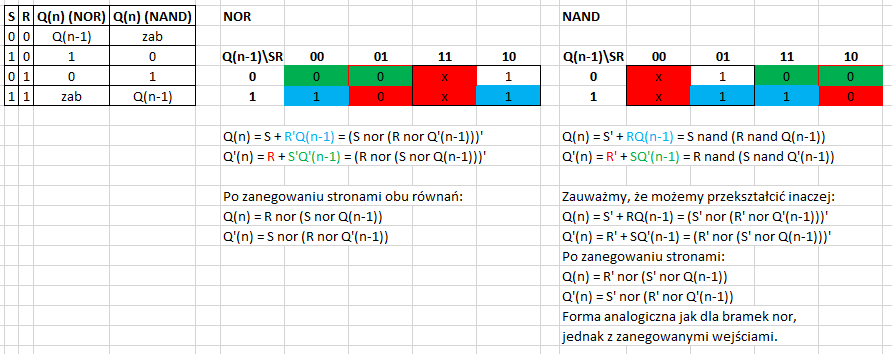
\includegraphics[width=\textwidth]{img/3a_karnaugh}
\end{figure}
\begin{figure}[H]
\centering
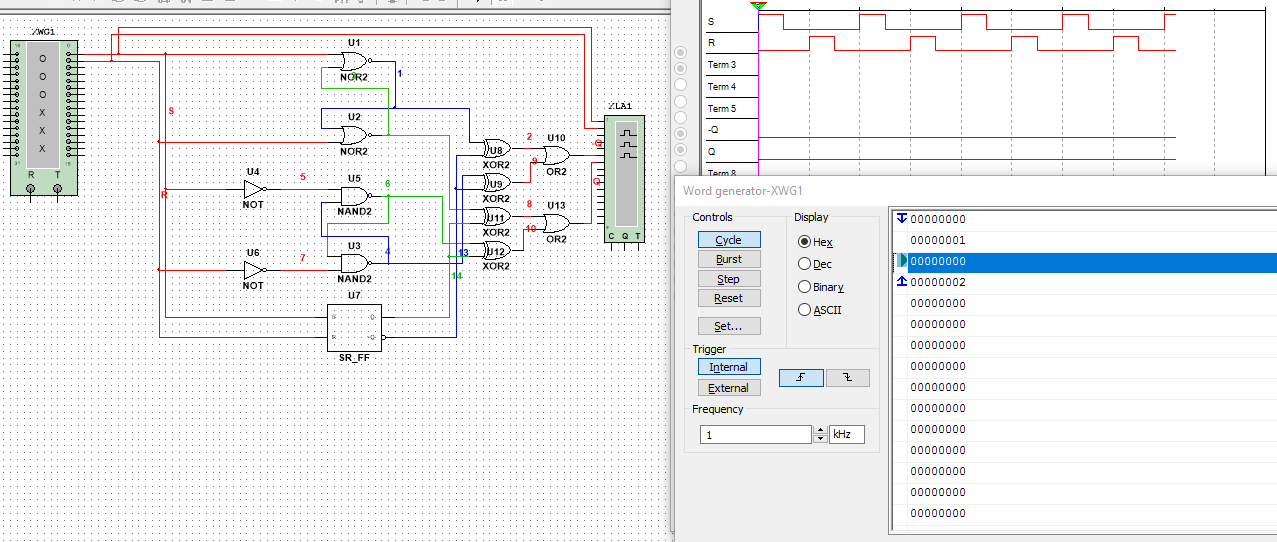
\includegraphics[width=\textwidth]{img/3a}
\end{figure}

Widzimy, że przerzutnik działa zgodnie z przewidywaniami. Przerzutnik oparty o bramki NAND działa tak, jakbyśmy zanegowali wejścia przerzutnika opartego o bramki NOR.

\subsection{Synchroniczny przerzutnik RS}
\begin{figure}[H]
\centering
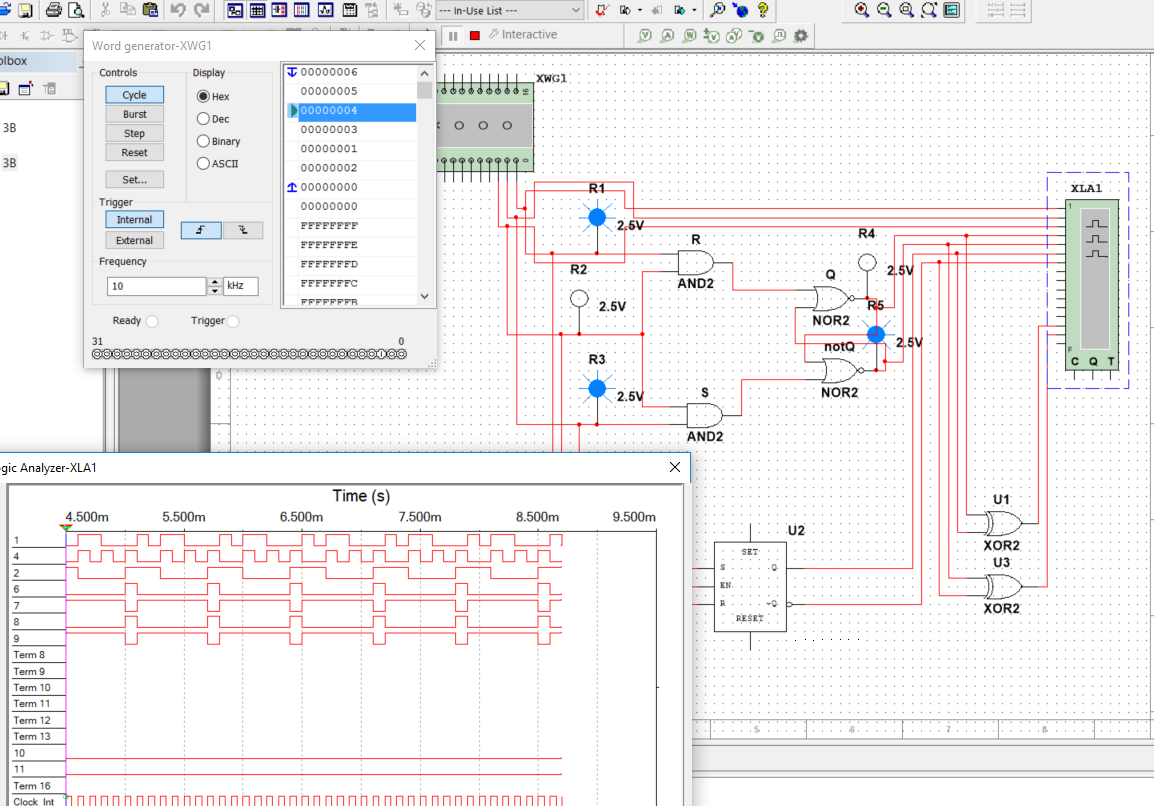
\includegraphics[width=\textwidth]{img/3b}
\end{figure}

\begin{figure}[H]
\centering
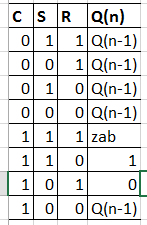
\includegraphics{img/3bTruthTable}
\end{figure}

Synchroniczny przerzutnik RS zmienia stan swoich wyjść tylko, gdy wejście zegara jest w stanie wysokim

Z analizy logic analyzerem widać, że zmontowany przerzutnik działa poprawnie. 

Synchroniczne przerzutniki RS są często stosowane przy taktowaniu sieci cyfrowych - dzięki temu można być pewnym, że ich elementy są ze sobą zsynchronizowane i skoordynowane.

\subsection{Synchroniczny przerzutnik JK}
\begin{figure}[H]
\centering
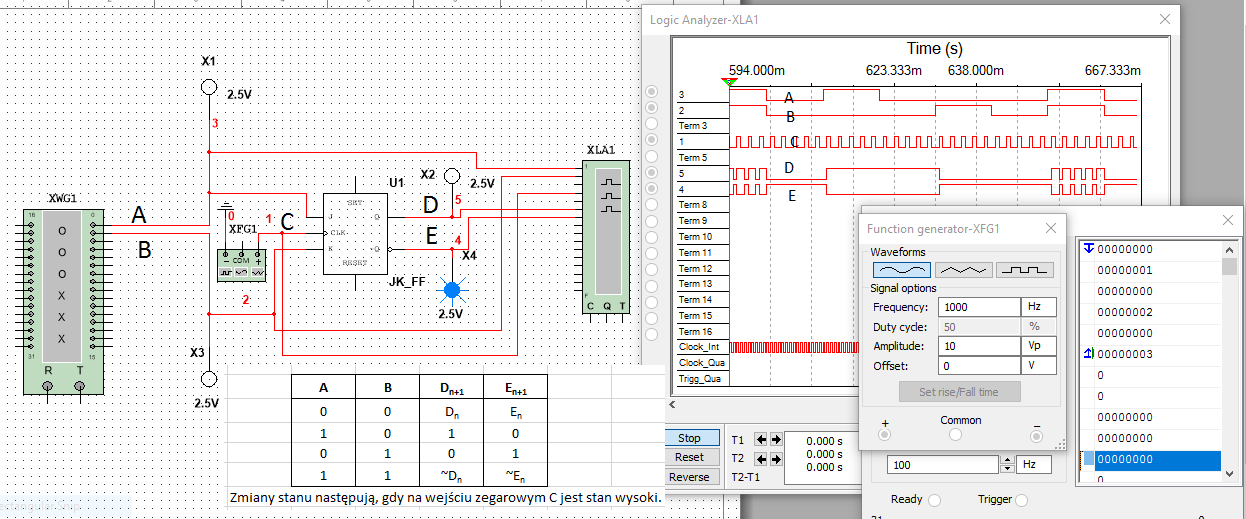
\includegraphics[width=\textwidth]{img/3c_syncJK}
\end{figure}

\begin{figure}[H]
\centering
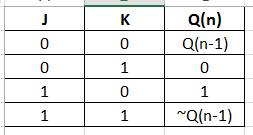
\includegraphics{img/3cTruthTable}
\end{figure}

Przerzutnik JK ma dwa wejścia:
\begin{itemize}
\item jedynkujące
\item kasujące
\end{itemize}

Jest on również synchroniczny. Jego działanie opisuje  powyższa tabela prawdy. Jak widać na załączonym schemacie, przetestowanie tej tablicy w Multisimie zakończyło się sukcesem.


Ciekawostka: nazwa przerzutnika pochodzi od inicjałów  \textbf{Jacka Kilby'yego} - wynalazcy układów scalonych (nie mylić z Jackiem Kirbym).


\subsection{Przerzutnik D na podstawie asynchronicznego przerzutnika RS}
\begin{figure}[H]
\centering
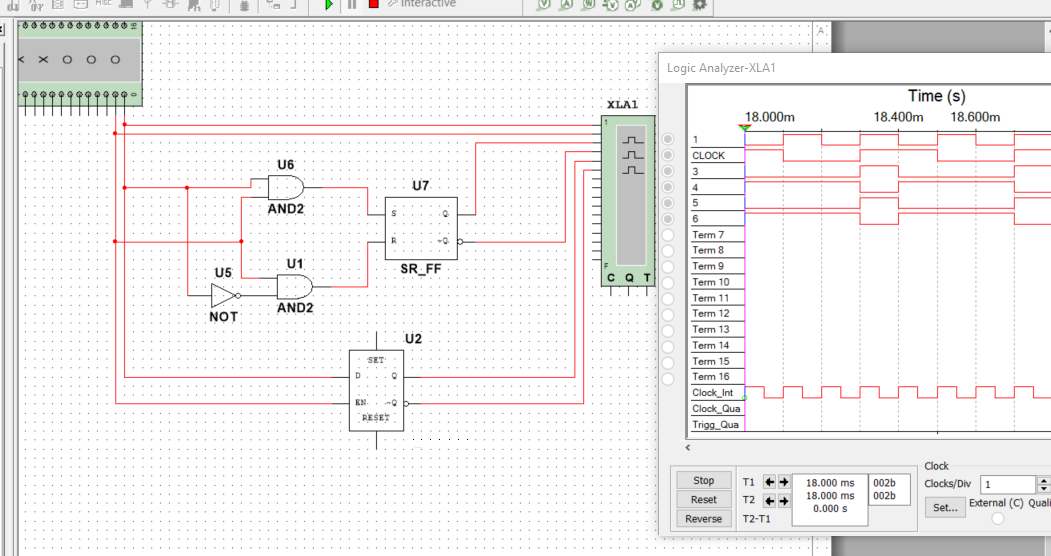
\includegraphics[width=0.3\textwidth]{img/3d}
\end{figure}
\begin{figure}[H]
\centering
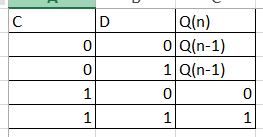
\includegraphics[width=0.3\textwidth]{img/3dTruthTable}
\end{figure}

Nazwa przerzutnika pochodzi z j. angielskiego - od słowa \textit{data} lub \textit{delay}. Jest to układ opóźniający - przepisuje sygnał wejściowy, ale tylko przy odpowiednim sygnale zegara. Jest to zatem także układ synchroniczny.

Przerzutnik D znajduje szerokie zastosowanie w budowie rejestrów.

\subsection{Przerzutnik T na podstawie synchronicznego przerzutnika D}
%\begin{figure}[H]
%\centering
%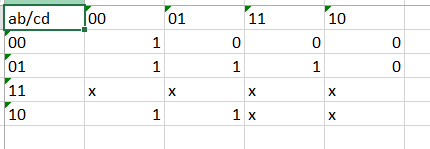
\includegraphics[width=0.3\textwidth]{7seg/seg1}
%\end{figure}

Przerzutnik typu T (eng. \textit{Toggle}), który po podaniu stanu wysokiego na wejście T i opadnięciu sygnału zegarowego zmienia stan wyjścia na przeciwny od dotychczasowego.



\subsection{Przerzutnik D na podstawie synchronicznego przerzutnika JK}
\begin{figure}[H]
\centering
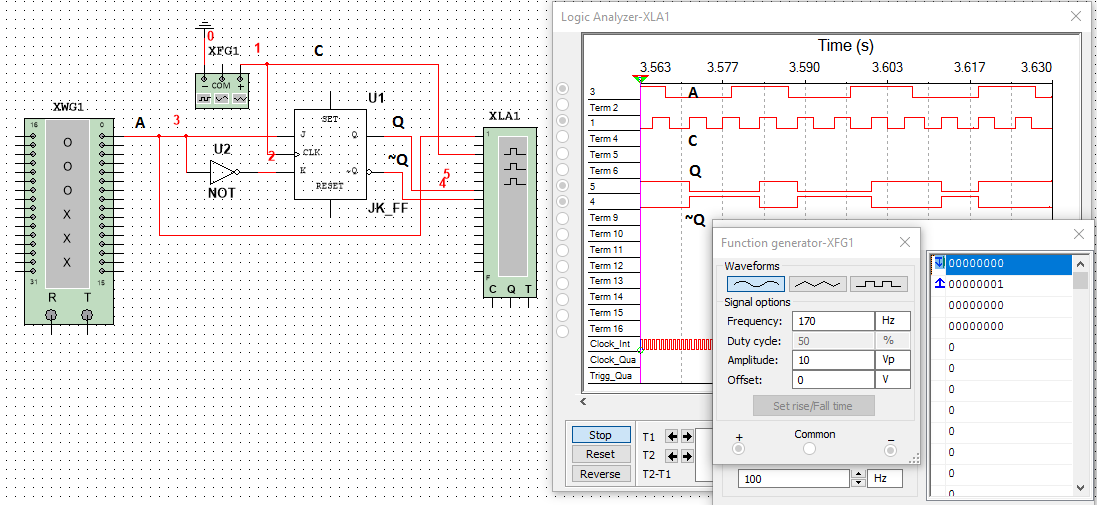
\includegraphics[width=\textwidth]{img/3f}
\end{figure}
\begin{figure}[H]
\centering
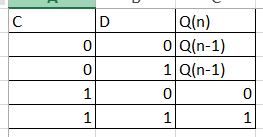
\includegraphics[width=0.3\textwidth]{img/3dTruthTable}
\end{figure}

Powyższy układ ilustruje budowę przerzutnika D za pomocą przerzutnika JK. Jak widać, inżynierzy elektronicy mają w budowie swoich układów do dyspozycji często całe wachlarze możliwości konstrukcyjnych dla zrealizowania tych samych potrzeb.


\subsection{Przerzutnik T na podstawie synchronicznego przerzutnika JK}
\begin{figure}[H]
\centering
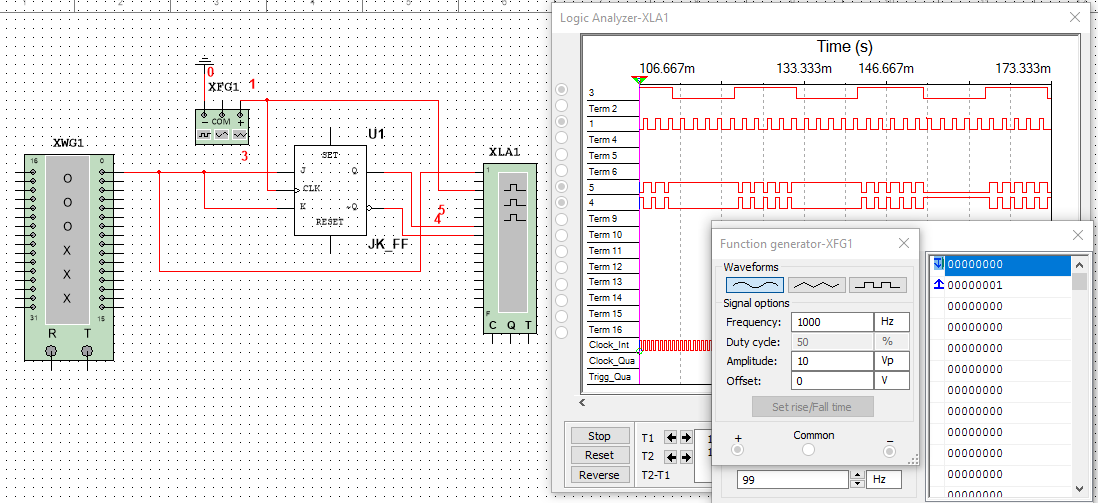
\includegraphics[width=\textwidth]{img/3g}
\end{figure}

Powyższy układ ilustruje budowę przerzutnika T za pomocą przerzutnika JK. 

Jak widać z powyższego i poprzedniego przykładu, prosty układ JK może być podstawą wielu przerzutników pełniących cały szereg różnych funkcji. 
\subsection{Rejestry na podstawie synchronicznych przerzutników D}

\subsubsection{Rejestr PIPO}
\begin{figure}[H]
\centering
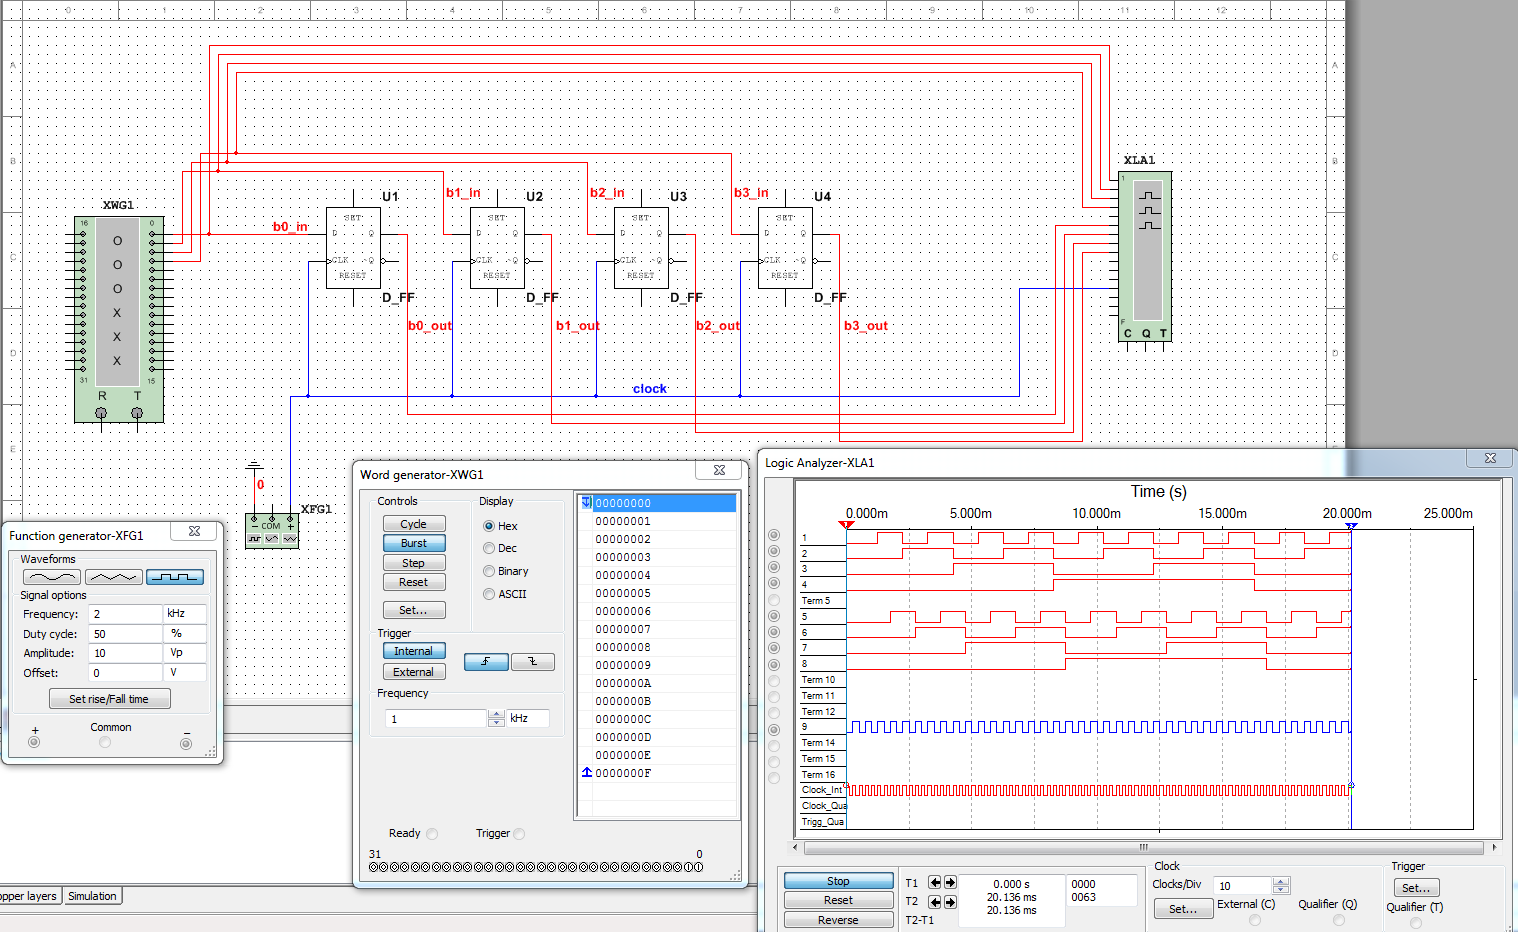
\includegraphics[width=\textwidth]{img/3hPIPO}
\end{figure}
\textbf{PIPO - Parallel-In Parallel-Out} - równoległe wejścia i równoległe wyjścia, czyli wejście i wyjście rejestru jest "szyną" 4 bitową - w każdym z przerzutników sygnał zmieniany jest tylko, gdy dany jest odpowiedni sygnał z zegara.

\subsubsection{Rejestr SIPO}
\begin{figure}[H]
\centering
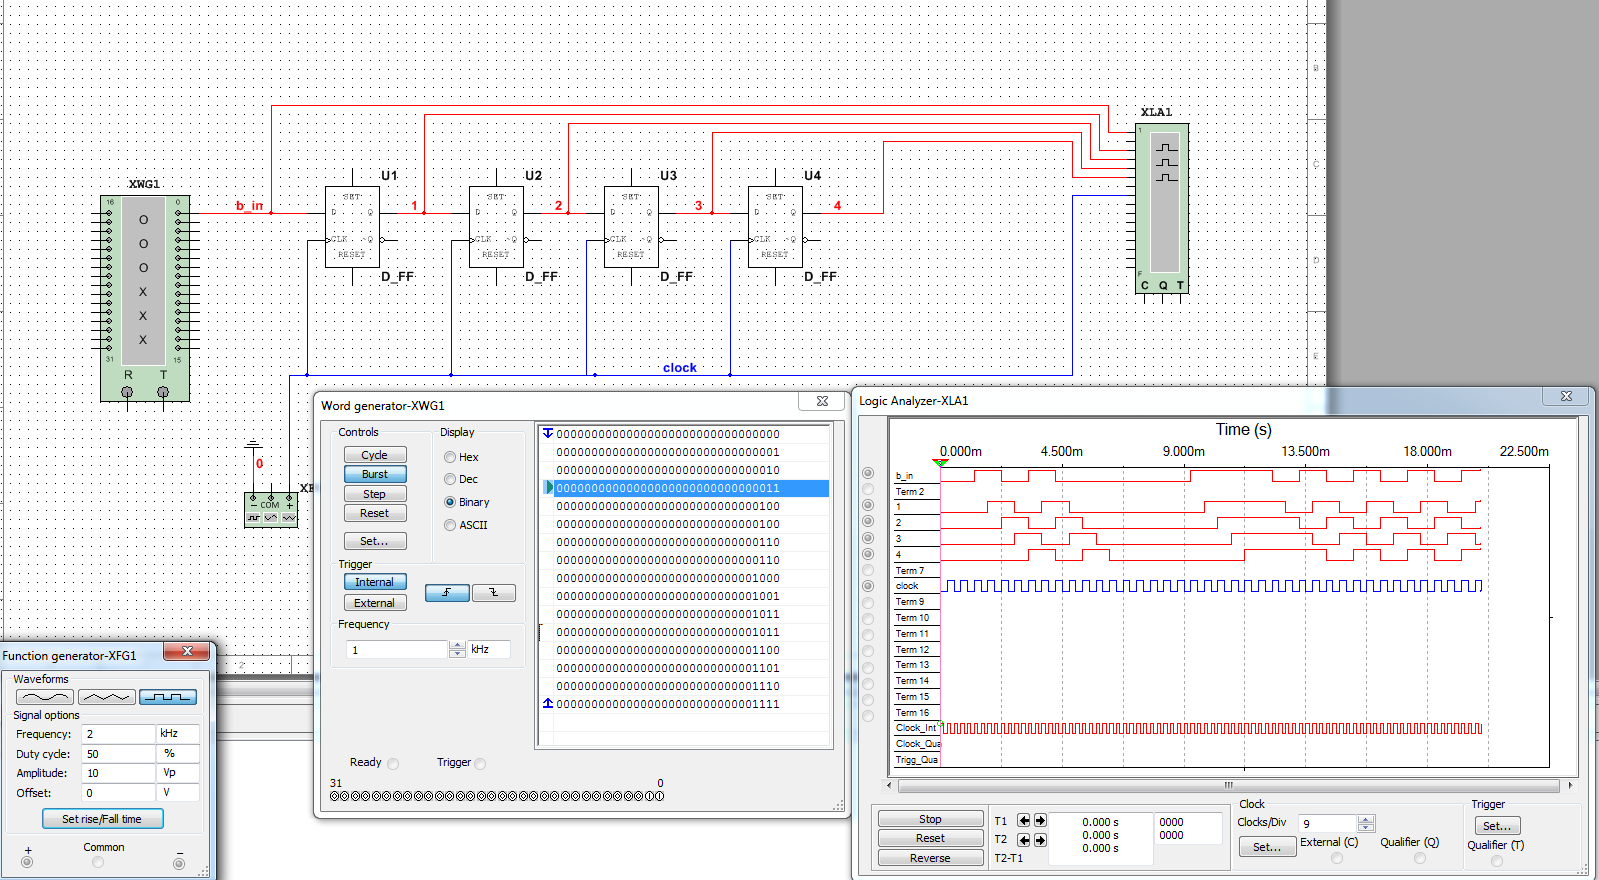
\includegraphics[width=\textwidth]{img/3hSIPO}
\end{figure}

\textbf{SIPO - Serial-In Parallel-Out} - szeregowe wejście, równoległe wyjście - na pojedynczym wejściu podajemy ciąg bitów, a na wyjściu dostajemy 4 równoległe bity. Wejście każdego kolejnego przerzutnika D podłączamy do wyjścia poprzedniego, wejście pierwszego z nich podłączamy do źródła danych. Wyjście każdego z przerzutników to kolejne bity wyjścia rejestru. Z każdym kolejnym cyklem zegara bity przesuwają się w prawo.
Bit najbardziej po prawej jest tracony, najbardziej po lewej jest odczytywany z wejścia szeregowego.

\subsubsection{Rejestr PISO}
\begin{figure}[H]
\centering
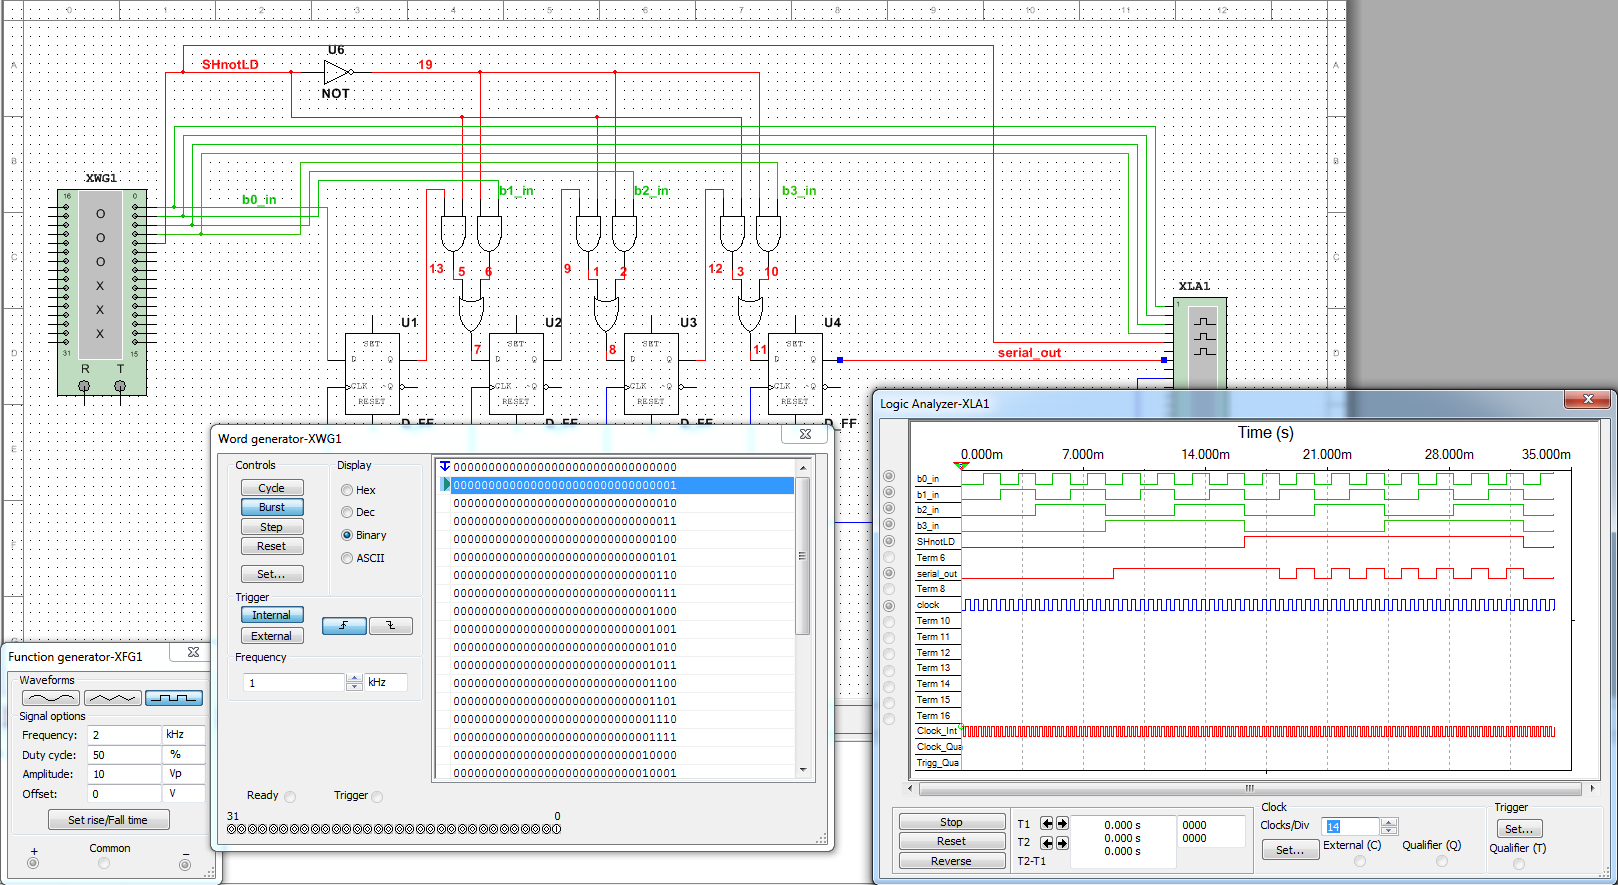
\includegraphics[width=\textwidth]{img/3hPISO}
\end{figure}

\textbf{PISO - Parallel-In Serial-Out} - na wejściu podajemy wiele sygnałów (równolegle), zaś na wyjściu otrzymujemy sygnał szeregowy. Potrzebna jest  możliwość wybrania - czy przesuwamy liczbę w rejestrze w prawo, czy też wczytujemy nową liczbę do rejestru wieloma wejściami. Osiąga się to następującą metodą:


Korzystamy z elementu o nazwie multiplekser - na wejściu dostaje on sterujący sygnał jednobitowy i dwa sygnały jednobitowe (źródła), między którymi będzie przełączał. W zależności od wartości sygnału sterującego, na wyjściu multipleksera pojawia się albo sygnał z jednego źródła, albo z drugiego. Na funkcji - jeżeli oznaczymy sygnał sterujący przez C, wejścia przez A, B, to multiplekser jednobitowy realizuje funkcję Y = AC + B(~C), czyli jeżeli C==1, na wyjściu jest A, jeżeli C==0, na wyjściu jest B.
W tym wypadku jednym ze źródeł jest wyjście poprzedniego rejestru (bo chcemy móc przesuwać bity w rejestrze), a drugim jest wejście danych (czyli miejsce, skąd chcemy wpisać dane do rejestru). 
Do każdego wejścia równoległego oprócz pierwszego dodajemy taki multiplekser. Sygnałem sterującym jest SHnotLD - jeżeli sygnał sterujący jest wysoki to wykonujemy SHift - przesunięcie, a jeżeli jest niski, to wykonujemy LoaD - załadowanie nowej liczby do rejestru.

\subsubsection{Rejestr SISO}
\begin{figure}[H]
\centering
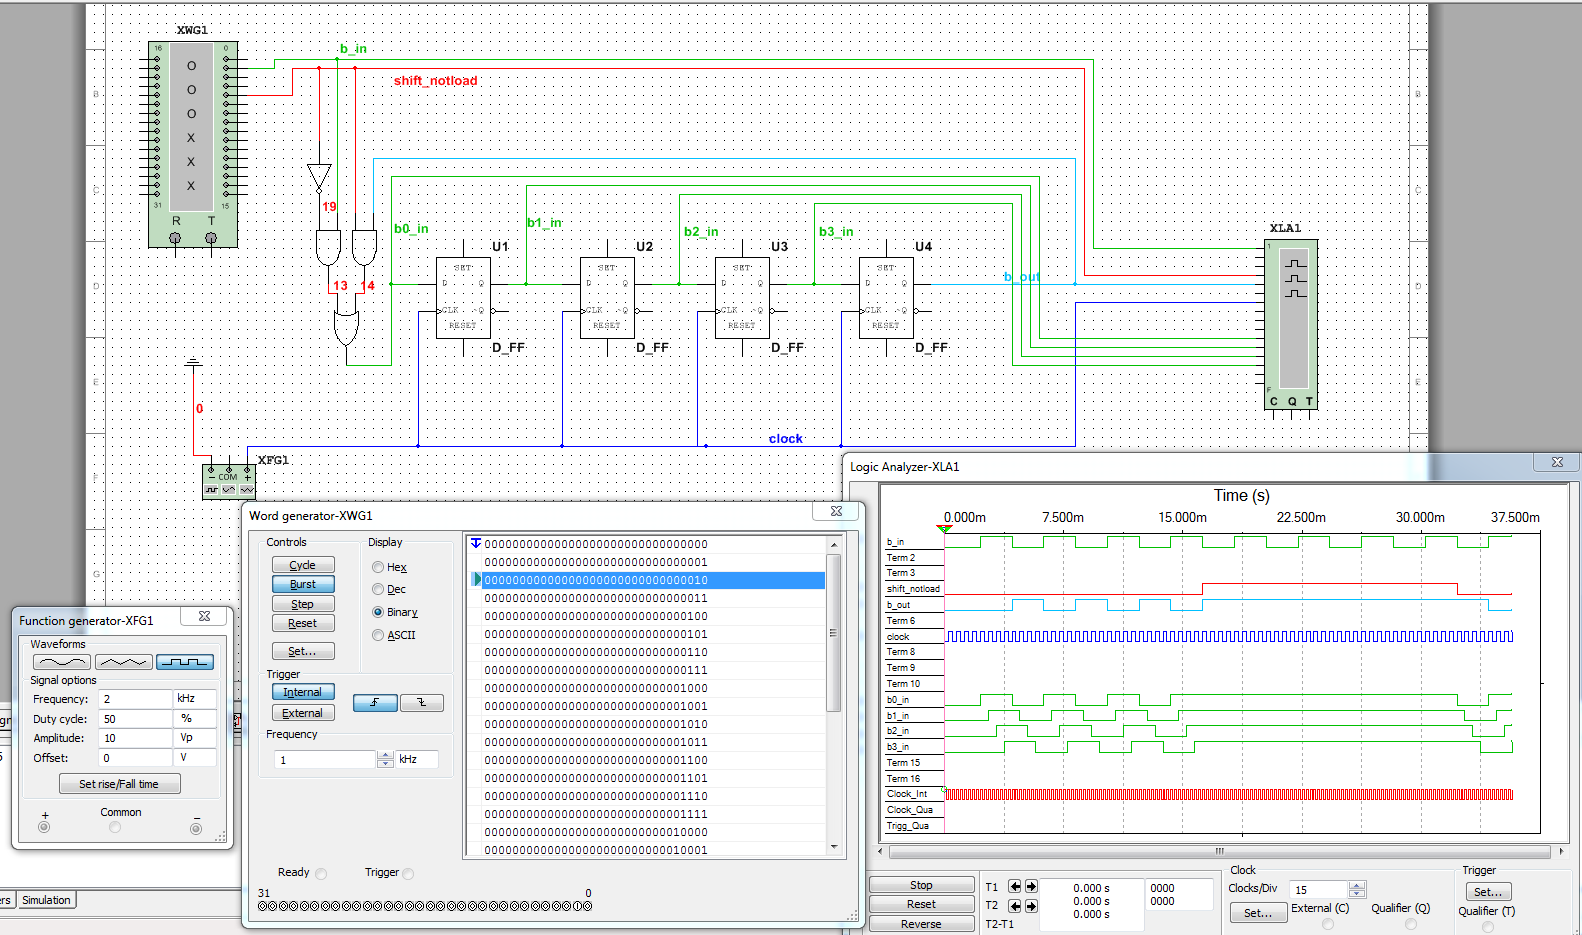
\includegraphics[width=\textwidth]{img/3hSISO}
\end{figure}

\textbf{SISO - Serial-In Serial-Out} - ten rejestr szeregowo dostaje dane i szeregowo ma je zwrócić. Ponieważ na wejściu dostajemy cały czas jakiś sygnał, to chcemy zapobiec utracie to, co w rejestrze jest. Dlatego tutaj też stosujemy multiplekser korzystający z sygnału SHnotLD, tym razem jednak używamy go, żeby "zapętlić" wyjście szeregowe z wejściem. Wtedy sygnałem SHnotLD, wybieramy czy przesuwamy dalej dane w prawo gubiąc stare (dla sygnału 1 SHnotLD), czy też zapętlamy wyjście z wejściem, czyli efektywnie to co było w rejestrze, będzie się w nim zapętlać.



\section{Wnioski}
Dzięki temu ćwiczeniu dowiedzieliśmy się, jak przerzutniki mogą posłużyć ku wyjściu na kolejny poziom abstrakcji - do zbudowania rejestrów, skąd już tylko niewielki krok do asemblera i języków wysokiego poziomu.

\end{document}
